\documentclass[11pt]{amsart}
\usepackage{geometry}                % See geometry.pdf to learn the layout options. There are lots.
\geometry{letterpaper}                   % ... or a4paper or a5paper or ... 
%\geometry{landscape}                % Activate for for rotated page geometry
%\usepackage[parfill]{parskip}    % Activate to begin paragraphs with an empty line rather than an indent
\usepackage{graphicx}
\usepackage{amssymb}
\usepackage{epstopdf}
\usepackage[usenames,dvipsnames]{color}
\usepackage{fancyvrb}
\usepackage{listings}
\usepackage{booktabs,footmisc}
\usepackage{hyperref}
\usepackage[all]{hypcap}

\usepackage{topcapt}


 
% include the lines below to use a nicer fixed-width font than the default one
 
\lstset{fancyvrb=true}
\lstset{
	basicstyle=\small\tt,
	identifierstyle=,
	commentstyle=\color{Bittersweet},
	stringstyle=\color{red},
	showstringspaces=false,
	tabsize=3,
	numbers=left,
	captionpos=b,
	xleftmargin=2em
%	numberstyle=\tiny
	%stepnumber=4
	}
\DeclareGraphicsRule{.tif}{png}{.png}{`convert #1 `dirname #1`/`basename #1 .tif`.png}

\title{Repast Model Testing Guide}
\author{Jonathan Ozik, Nick Collier - Repast Development Team}
\date{\today}                                           % Activate to display a given date or no date

\begin{document} 
\maketitle
\setcounter{section}{-1}

\section{Before we Get Started}
Before we can do anything with Repast Simphony, we need to make sure that we have a proper installation of Repast Simphony 2.2. Instructions on downloading and installing Repast Simphony on various platforms can be found on the \href{http://repast.sourceforge.net/download.html}{Repast website}.\footnote{http://repast.sourceforge.net/download.html} Repast Simphony 2.2 requires Java 7. Java 7 can be found at the \href{http://www.oracle.com/technetwork/java/javase/downloads/index.html}{Java Standard Edition Downloads Page}.\footnote{http://www.oracle.com/technetwork/java/javase/downloads/index.html}


\section{Getting Started with Repast Simphony Model Testing}

Developing a useful agent-based simulation involves acquiring sufficient knowledge of a model�s domain, developing the conceptual model, often while grounding it in more abstract theories of the domain, and then translating the model into software. The work can be complex and is rarely a waterfall type process where each step is completed before the next step begins. Rather, the process in an iterative one where the development of the model may require additional domain knowledge that, in turn, requires changes in the software. Furthermore, model specifications and requirements may change also requiring changes in the software. Test-driven development (TDD) is a general software development technique that can help with managing this complexity. In TDD the development of software is driven by the creation of many small automated unit tests each of which exercise some small part of the larger system's behavior. An aspect of the extreme-programming movement that has gained popularity since the late 1990s, the technique itself gained in prominence with the publication of Kent Beck's seminal work ``Test-Driven Development: By Example"\footnote{Beck, K. 2003. Test Driven Development: By Example. Boston, Massachusetts: Addison-Wesley.}.

The present guide will walk you through a number of agent-model TDD use cases with Repast Simphony. For those interested in learning more about agent-model testing, including the benefits of TDD when developing agent models, see Collier and Ozik (2013)\footnote{Collier, N, and J Ozik. �Test-Driven Agent-Based Simulation Development.� To appear in WSC 2013 Proceedings. Washington, D.C., 2013.}. For more information on the JUnit testing framework that we will be using, see \href{http://junit.org}{http://junit.org}.

\section{Agent-model Testing Use Cases with Repast Simphony}
To add tests into an existing Repast Simphony project, we recommend the following setup steps:
\begin{enumerate}
\item
Add a \texttt{test} source folder to the project. This can be accomplished in a number of ways. One way is to right click on the project and navigate to \emph{New} $\rightarrow$ \emph{Source Folder} (Fig.~\ref{fig:newSourceFolder}). Then fill in \texttt{test} in the \emph{Folder name} text field and click on \emph{Finish} (Fig.~\ref{fig:testSourceFolder}).

\begin{figure}
\begin{center}
\vspace{.2in}
\centerline {
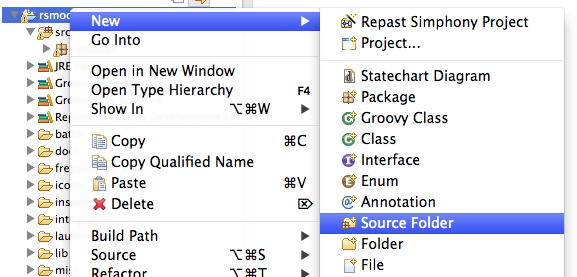
\includegraphics[width=4in]{RepastModelTestingImages/NewSourceFolder.png}
}
\caption{Selecting your project, right-clicking and choosing \emph{New} $\rightarrow$ \emph{Source Folder}.}
\label{fig:newSourceFolder}
\end{center}
\end{figure}

\begin{figure}
\begin{center}
\vspace{.2in}
\centerline {
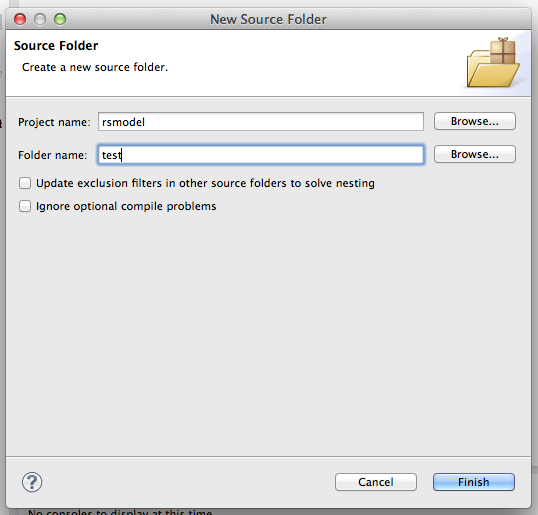
\includegraphics[width=4in]{RepastModelTestingImages/testSourceFolder.png}
}
\caption{New source folder wizard.}
\label{fig:testSourceFolder}
\end{center}
\end{figure}

\item
Modify the output folder for the \texttt{test} source folder. Right click on the project and navigate to \emph{Properties}. Then choose the \emph{Java Build Path} entry in the left bar and select the \emph{Source} tab. Select the check box that reads \emph{Allow output folders for source folders} and expand the \texttt{test} entry (Fig.~\ref{fig:javaBuildPath}). Select the \emph{Output folder} entry and click on the \emph{Edit} button (Fig.~\ref{fig:EditOutputFolder}). Then select the \textit{Specific output folder} option and input \texttt{testbin}, or something else different from \texttt{bin} (Fig.~\ref{fig:SourceFolderOutputLocation}). Click on \emph{Okay} and then \emph{Okay} again.

\begin{figure}
\begin{center}
\vspace{.2in}
\centerline {
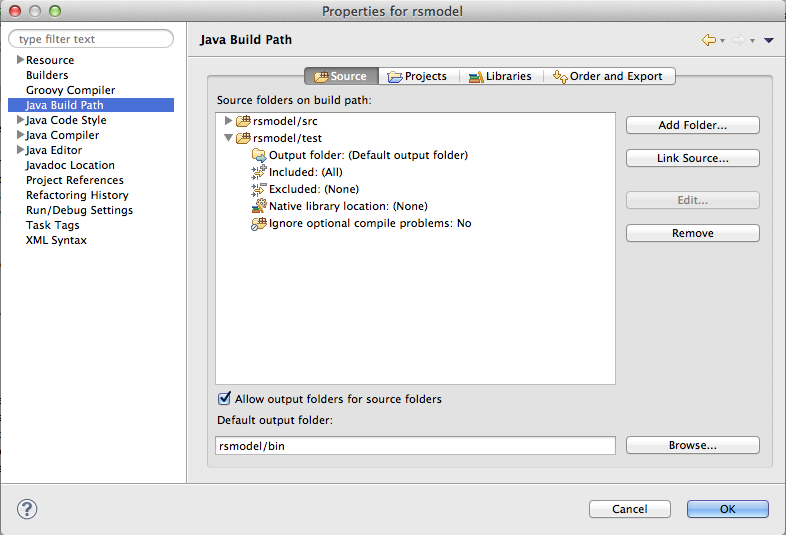
\includegraphics[width=4in]{RepastModelTestingImages/javaBuildPath.png}
}
\caption{\emph{Java Build Path} $\rightarrow$ \emph{Source} tab in a project's properties.}
\label{fig:javaBuildPath}
\end{center}
\end{figure}

\begin{figure}
\begin{center}
\vspace{.2in}
\centerline {
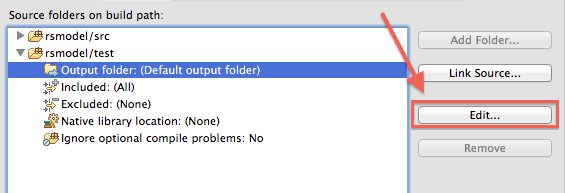
\includegraphics[width=4in]{RepastModelTestingImages/EditOutputFolder.png}
}
\caption{Edit the output folder of the \texttt{test} source folder.}
\label{fig:EditOutputFolder}
\end{center}
\end{figure}

\begin{figure}
\begin{center}
\vspace{.2in}
\centerline {
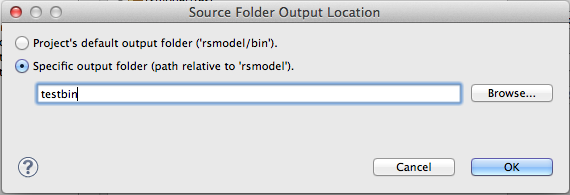
\includegraphics[width=4in]{RepastModelTestingImages/SourceFolderOutputLocation.png}
}
\caption{Choosing the source folder output location.}
\label{fig:SourceFolderOutputLocation}
\end{center}
\end{figure}


\item
Add a JUnit Test Case by right clicking on the project in the Package Explorer view,  choosing \emph{New} $\rightarrow$ \emph{Other}\ldots (Fig.~\ref{fig:newOther}). Then navigate to \emph{Java} $\rightarrow$ \emph{JUnit} and choose \emph{Junit Test Case} (Fig.~\ref{fig:JUnitTestCase})\footnote{This creates a Java JUnit test case, but a Groovy JUnit test case can be used as well.}. In the \emph{New JUnit Test Case} wizard choose the \emph{New JUnit 4 test} option, specify the correct source folder (\texttt{test}), name your test case, include all the method stubs, and click on \emph{Finish} (Fig.~\ref{fig:NewJUnitTestCase})\footnote{While this document is focused on JUnit 4, JUnit 3 or other testing frameworks can also be utilized.}. If JUnit was not previously on your project's build path, you will see a dialog asking if you'd like to add it (Fig.~\ref{fig:AddToBuildPath}). Click \emph{OK} to add the JUnit 4 library to the project's build path.

\begin{figure}
\begin{center}
\vspace{.2in}
\centerline {
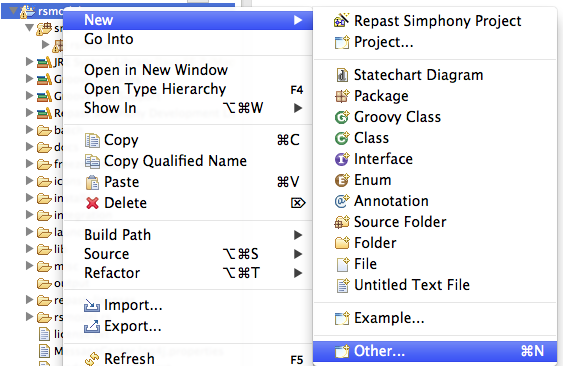
\includegraphics[width=4in]{RepastModelTestingImages/NewOther.png}
}
\caption{Selecting your project, right-clicking and choosing New $\rightarrow$ Other... .}
\label{fig:newOther}
\end{center}
\end{figure}

\begin{figure}
\begin{center}
\vspace{.2in}
\centerline {
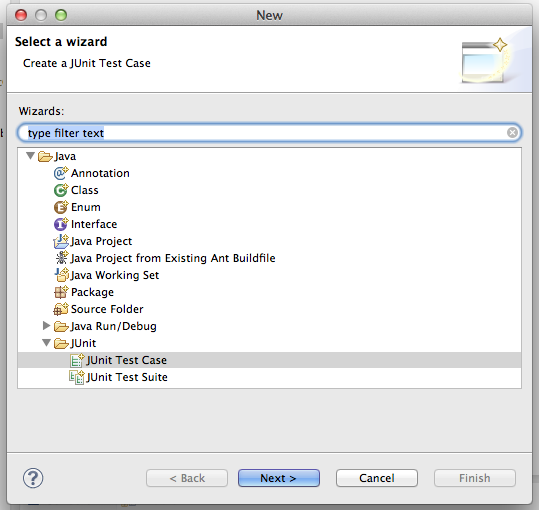
\includegraphics[width=4in]{RepastModelTestingImages/JUnitTestCase.png}
}
\caption{The JUnit Test Case option within Java $\rightarrow$ JUnit.}
\label{fig:JUnitTestCase}
\end{center}
\end{figure}

\begin{figure}
\begin{center}
\vspace{.2in}
\centerline {
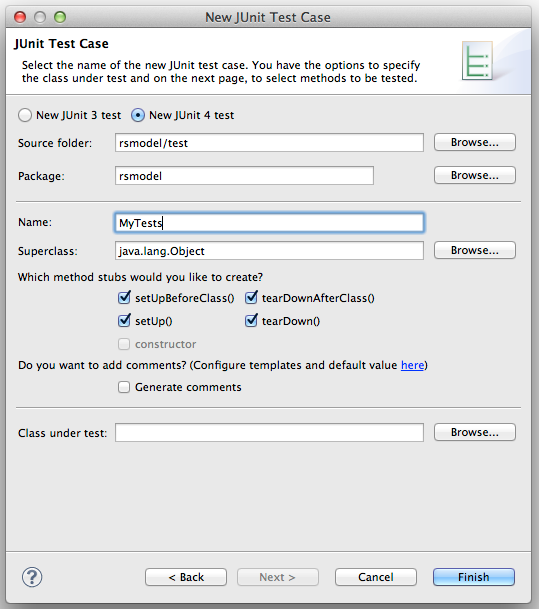
\includegraphics[width=3in]{RepastModelTestingImages/NewJUnitTestCase.png}
}
\caption{The new \emph{JUnit Test Case} wizard.}
\label{fig:NewJUnitTestCase}
\end{center}
\end{figure}

\begin{figure}
\begin{center}
\vspace{.2in}
\centerline {
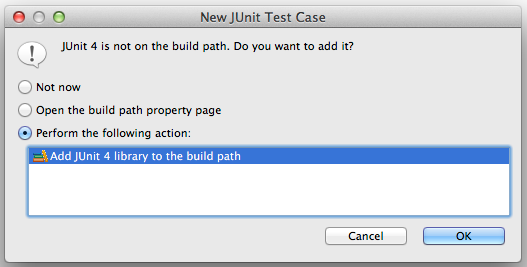
\includegraphics[width=4in]{RepastModelTestingImages/AddToBuildPath.png}
}
\caption{Add JUnit 4 library to build path.}
\label{fig:AddToBuildPath}
\end{center}
\end{figure}

\end{enumerate}
\clearpage

Once the setup is complete, there are a number of different types of model tests that can be created, based on the nature of the model behavior that is being tested. We will go over a few such cases next.

\subsection{Use Case 1: Simple Unit Testing with Repast Simphony Models}
If the elements being tested are relatively decoupled, there is nothing special that needs to be done in terms of test case setup. In this scenario, the @BeforeClass, @AfterClass, @Before, and @After annotated methods do not need any Repast Simphony specific elements and tests can be written in the usual way JUnit tests are written.

\subsection{Use Case 2: Schedule Based Model Testing with Repast Simphony Models}
\label{sec:use2}
Some model behaviors that you might want to test involve scheduled behaviors. For example, you might want to know that at a certain tick, specific model actions had occurred. This is especially relevant to any Statecharts related behaviors. In this situation, the RunEnvironment will need to be passed a Schedule object. Listing~\ref{lst:scheduleSetup} shows an example where the schedule based setup is executed before each of the tests that will be run (i.e., in the @Before annotated method).
 
\noindent\begin{minipage}[h]{\textwidth}
\vspace{.2in}
\lstset{language=java,caption=@Before setup method in a schedule dependent test case.,label=lst:scheduleSetup}
\begin{lstlisting}
@Before
public void setUp() throws Exception {
	Schedule schedule = new Schedule();
	RunEnvironment.init(schedule, null, null, true);
	Context context = new DefaultContext();
	RunState.init().setMasterContext(context);
	
	// Any additional setup
}

\end{lstlisting}
\vspace{.2in}
\end{minipage}
Line 3 in Listing~\ref{lst:scheduleSetup} shows the creation of the Schedule object. It is then sent as the first parameter to the RunEnvironment static \texttt{init} method. The second and third parameters can be \texttt{null} for this case and the fourth parameter indicates whether this is a batch (i.e., headless) run, which it is so we specify \texttt{true}. Line 5 creates a new DefaultContext that is set as the master context of the \texttt{init}-ed RunState in line 6. Lines 5 and 6 are only strictly necessary for testing behaviors that rely on a master context being set, which is the case for Statecharts.

At this point, tests can be written such as in Listing~\ref{lst:scheduleSetupTest}:

\noindent\begin{minipage}[h]{\textwidth}
\vspace{.2in}
\lstset{language=java,caption=Example test method where the schedule is advanced.,label=lst:scheduleSetupTest}
\begin{lstlisting}
@Test
public void testUninfectedToInfected() {
	ISchedule schedule = RunEnvironment.getInstance().
			getCurrentSchedule();
	Person p = new Person();
	assertEquals(UNINFECTED, p.getStatus());
	for (int i = 0; i < 5; ++i) {
		schedule.execute();
	}
	assertEquals(INFECTED, p.getStatus());
}
\end{lstlisting}
\vspace{.2in}
\end{minipage}
In this hypothetical example, a Person agent is created, it is verified that the person's status is \texttt{UNINFECTED}, the schedule is advanced 5 times, at which point the person's status is checked to see that it is \texttt{INFECTED}. An important item to note here is that the scheduler in Repast Simphony doesn't just allow for discrete time steps so the fact that the schedule is executed 5 times doesn't necessarily mean that we will find ourselves at tick 5 after the \texttt{for} loop, unless there were actions scheduled only to occur on every tick.

\subsection{Use Case 3: Context Builder Based Model Testing with Repast Simphony Models}
\label{sec:use3}
For cases where the specific setup defined in a ContextBuilder is required for testing, the @Before testing setup might look like Listing~\ref{lst:contextBuilderSetup}.

\noindent\begin{minipage}[h]{\textwidth}
\vspace{.2in}
\lstset{language=java,caption=@Before setup method in a context builder dependent test case.,label=lst:contextBuilderSetup}
\begin{lstlisting}
. . .
public Context context;

@Before
public void setUp() throws Exception {
	context = new DefaultContext();
	MyContextBuilder builder = new MyContextBuilder();
	context = builder.build(context);
	
	// Any additional setup
}
. . .
\end{lstlisting}
\vspace{.2in}
\end{minipage}
Here, after creating the DefaultContext, the context builder is used to build it into the state it should be in at the start of each simulation run. A test utilizing the setup in Listing~\ref{lst:contextBuilderSetup} might look like Listing~\ref{lst:contextBuilderSetupTest}. In this hypothetical test, a new Person agent is added to the main context and a \texttt{hasNeighbors} method is called to ensure that the added Person agent has neighbors in the pre-built context.

\noindent\begin{minipage}[h]{\textwidth}
\vspace{.2in}
\lstset{language=java,caption=Example test method where the context state created by a context builder is used.,label=lst:contextBuilderSetupTest}
\begin{lstlisting}
@Test
public void testAddingPersonToContext() {
	Person p = new Person();
	context.add(p);
	assertTrue(p.hasNeighbors());
}
\end{lstlisting}
\vspace{.2in}
\end{minipage}


\subsection{Use Case 4: Model Testing with ReLogo Models}
ReLogo models come with the infrastucture and associated assumptions of the ReLogo world which is built by the SimBuilder context builder included with each model. To test a ReLogo model there are a few additional steps needed for the test setup beyond what was done in Section~\ref{sec:use3}. Listing~\ref{lst:relogoSetup} shows the setup (optionally) separated into @BeforeClass and @Before components. The idea here is that the ReLogo world is built once before all the tests are run but before each individual test is executed, the observer clears the ReLogo world state, removing existing turtles and links and resetting patches.

\noindent\begin{minipage}[h]{\textwidth}
\vspace{.2in}
\lstset{language=java,caption=@Setup method in a schedule dependent test case.,label=lst:relogoSetup}
\begin{lstlisting}
. . .
static UserObserver observer;

@BeforeClass
public static void setUpBeforeClass() throws Exception {
	String scenarioDirString = "ModelName.rs";
	ScenarioUtils.setScenarioDir(new File(scenarioDirString));
	File paramsFile = new File(ScenarioUtils.getScenarioDir(),
		"parameters.xml");
	ParametersParser pp = new ParametersParser(paramsFile);
	Parameters params = pp.getParameters();
	RunEnvironment.init(new Schedule(), null, params, true);
	Context context = new DefaultContext();
	SimBuilder builder = new SimBuilder();
	context = builder.build(context);
	
	// If statecharts are used in the ReLogo model
	RunState.init().setMasterContext(context);
	
	observer = (UserObserver)context.iterator().next();
	
	// Any additional before class setup
}

@Before
public void setUp() throws Exception {
	observer.clearAll();

	// Any additional setup
}
. . .
\end{lstlisting}
\vspace{.2in}
\end{minipage}
Some of the contents of Listing~\ref{lst:relogoSetup} will already look familiar from the previous sections but there are additions that we expand on here:
\begin{enumerate}
\item
The scenario directory (the .rs folder) is specified in Line 6. Replace ``ModelName.rs" with the name of the scenario directory in your project.
\item
The parameters.xml file within the scenario directory is parsed and passed to the RunEnvironment \texttt{init} method. This can be done in non-ReLogo models as well.
\item
If statecharts are used in the ReLogo model, Line 18 should be included as well.
\end{enumerate}
%Steps for creating harness: 
%create test source folder 
%output folder testbin 
%new package newproject.relogo in test source folder 
%new JUnit 4 test with all options checked (i.e., @BeforeClass, etc.) 
%
%Two examples to the right, one Java one Groovy. 
%Both can accept an "rsFolder" system property, e.g.: 
%
%-DrsFolder=${workspace_loc:NewProject}/NewProject.rs 
%
%Tried Spock but the dependencies weren�t convenient.


\end{document}  